% Performance testing +- same performance
% https://ieeexplore.ieee.org/abstract/document/8928192

% Performance testing +monolith
% https://ieeexplore.ieee.org/abstract/document/9109514

\section{Comparison}
Up to this point, we have walk through three different types of architecture patterns. In this section we are going to look into implementation of simple application using every pattern. We will look into implication concerning database design, scalability and of course performance.

\subsection{Application}
Application was design to be easy to understand and solve problem known to everyone: orders. Client can view items, add them to his shopping cart, place order, retrieve invoice and pay for it. As most of the applications today, there are mainly operations querying data or saving data into database. Activity flow is described on Diagram \ref{img:app_activity_flow}.

For implementation programming language the candidates were Rust and Golang due to its minimal runtime. Winner being Golang, because of it's easier usage, authors personal experience and better support for Open Tracing project, which will be used for monitoring during benchmarking. All applications are based on \textit{gorilla/mux} \cite{MUX} library for http server + request routing and \textit{Bun} \cite{BUN} as lightweight ORM.

PostgreSQL database was chosen as data storage, since SQL databases are more known compared to NoSQL, so it should be easier for everyone to understand the design. It was selected due to author preference over MySQL.
\begin{figure}
    \centering
    \includesvg{images/app_activity.svg}
    \caption{Diagram describes client flow of application. First session is created for client, then he load items and add all he wants into shopping cart. Later client places order, invoice is generated in background and client can cancel the order or pay for it. To add more cpu sensitive task, the generation of invoice generates pdf and also calculates 41st Fibonacci Number. \label{img:app_activity_flow}}
\end{figure}

\subsection{Monolith}
This example is implemented as Monolithic system. Basically it is Three-tier application: presentation (HTTP API), application and data (database). Diagram \ref{img:monolith_db_schema} describes internal application package structure. \textit{Routes} package contains path mapping for endpoints handlers defined in \textit{endpoints}. Handlers contain simple logic definition, more complex logic resides in \textit{services} and data manipulation around database is contained in \textit{database} package.

\begin{figure}
    \centering
    \includesvg[width=0.7\textwidth]{images/monolith_package.svg}
    \caption{Internal package structure of Monolithic example. \label{img:monolith_package}}
\end{figure}


\subsubsection{Database}
Due to nature of Monolith as unified system, all data resides inside single database fully leveraging constraints (e.g. foreign keys) and thus ensuring data consistency. Complete database schema is displayed on Diagram~\ref{img:monolith_db_schema} consisting of 7 tables, five of them for entity tables and two for entity relation mapping.

\begin{figure}
    \centering
    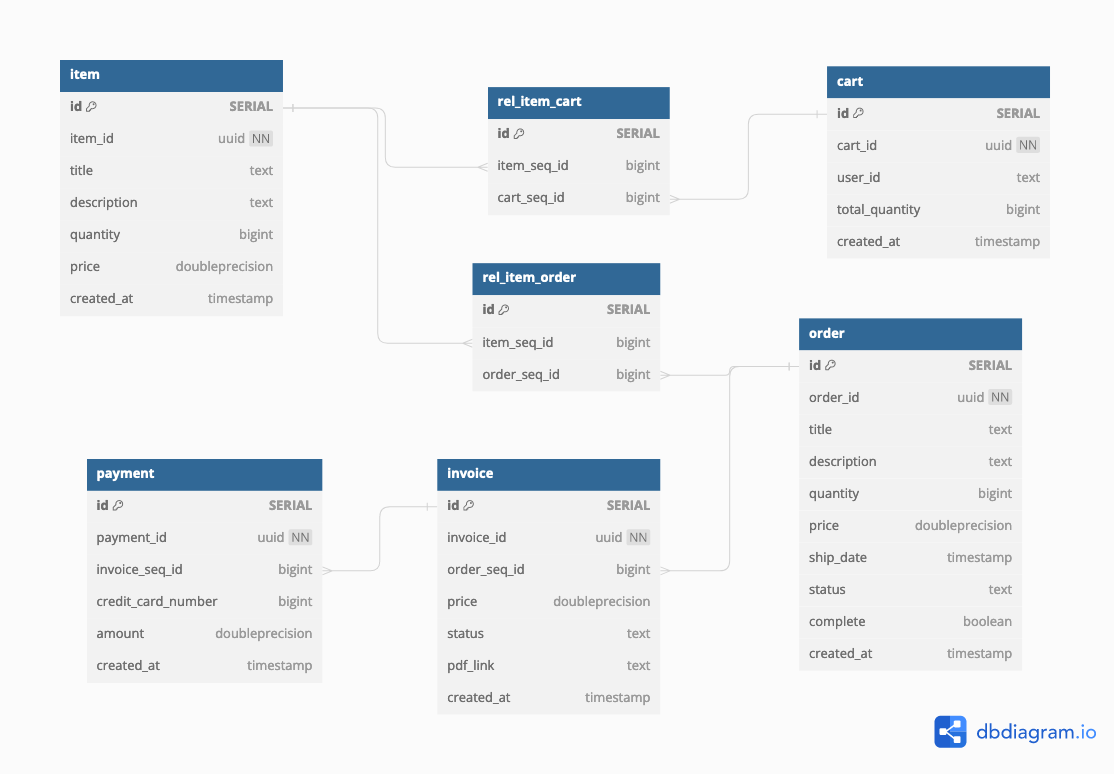
\includegraphics[width=\textwidth]{images/monolith_db_schema.png}
    \caption{Database schema displaying tables and relations of Monolithic example. \label{img:monolith_db_schema}}
\end{figure}



\subsection{Modulith 1}
This is example using Modular Monolith approach. The original Monolithic application was split into multiple smaller Monoliths called \textit{modules}. The scope of every module depends on the specificity of the project. In this case it nearly corresponds to module per Entity, exception being shopping cart and items, which were merged into single module to demonstrate possibility to have modules with different volume. Package schema and dependency is displayed on Diagram~\ref{img:modulith_package}

Every module has the same internal structure as original Monolith plus exposes its API with interface (Diagram~\ref{img:modulith_module_package}). Modules encapsulate its own data storage and there shouldn't be any inter-modules table constraint set in database, although it is possible, it does not make sense from the perspective of logical separation and might be very confusing. It should be possible for every module to use different database or and even different database technology.

Module can use API of other modules, although this should be limited as much as possible to keep coupling low. Dependency on other modules is defined through usage of interfaces and the actual implementation can be either injects automatically using IoC approach or as in this case just defining top level module, which takes care of initializing individual modules and spinning up HTTP server.

\begin{figure}
    \centering
    \includesvg[width=0.7\textwidth]{images/modulith_module_package.svg}
    \caption{Database schema displaying tables and relations. \label{img:modulith_module_package}}
\end{figure}

\begin{figure}
    \centering
    \includesvg[width=0.7\textwidth]{images/modulith_package.svg}
    \caption{Database schema displaying tables and relations. \label{img:modulith_package}}
\end{figure}

\subsubsection{Database}
Every module encapsulates its own tables completely independent of the rest. Table are the same as for Monolithic example on Diagram~\ref{img:monolith_db_schema}, but relation across modules were removed. The schema consist of four partitions with relations preserve in every partition: first invoice table, second payment, third order table with rel\_item\_order and last tables item, cart and rel\_item\_cart.

% \begin{figure}
%     \centering
%     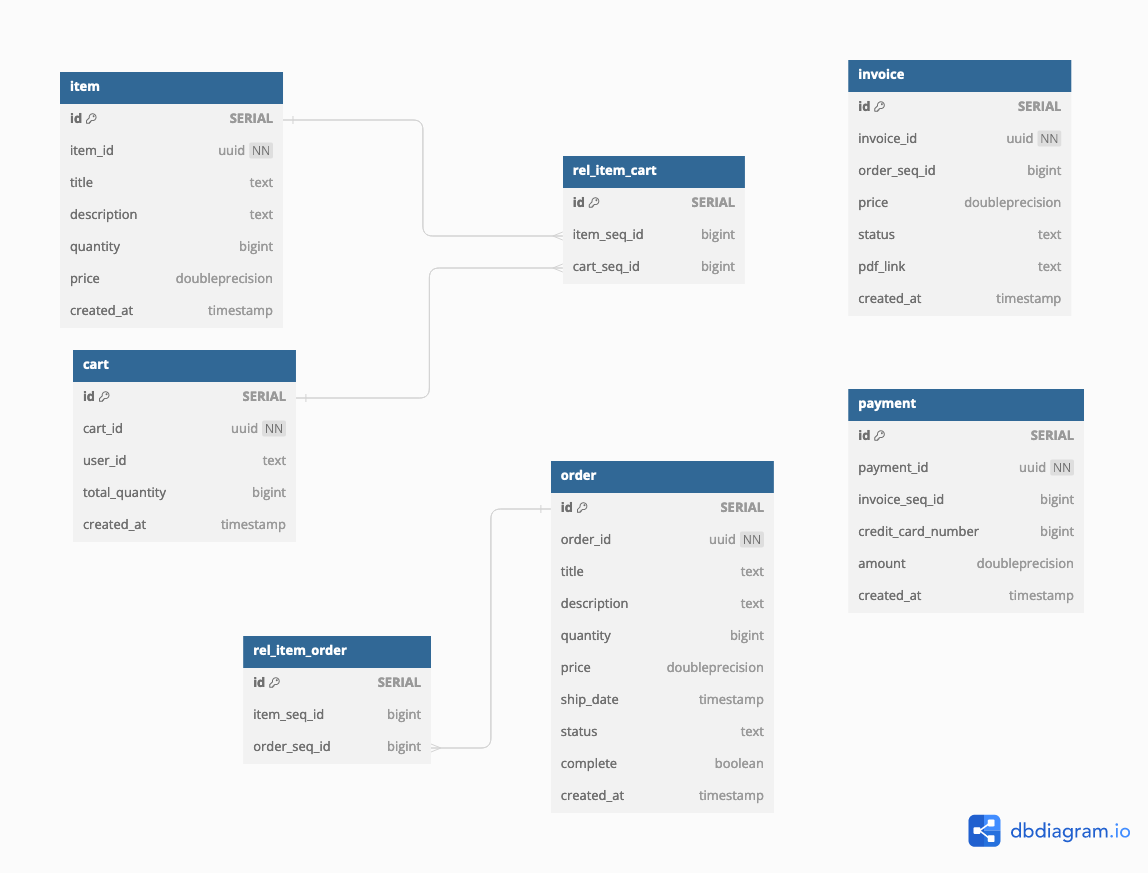
\includegraphics[width=\textwidth]{images/modulith_db_schema.png}
%     \caption{Database schema displaying tables and relations. \label{img:modulith_db_schema}}
% \end{figure}




\subsection{Benchmark methodology}
Specifications:
\begin{itemize}
    \item Golang 1.21.3
    \item PostgreSQL 14
    \item Docker 24.0.5
    \item Uptrace
    \item Hardware - TODO
\end{itemize}

% \subsection{Performance}

% latency
% throughput
% scalability
% 

% \subsection{Maintainability}
% Easy debugging | logging

% \subsection{Sustainability}
% transactions?

% \subsection{Testability}

% \subsection{Complexity}